\documentclass[11pt]{article}
\usepackage[utf8]{inputenc}
\usepackage[spanish]{babel}
\usepackage{graphicx}         % Para incluir imágenes
\usepackage{amsmath}          % Para notación matemática
\usepackage[margin=3cm]{geometry}  % Márgenes
\usepackage[font=normalsize,labelfont=small]{caption}  % Estilo de captions
\usepackage{hyperref}         % Para links clickeables
\usepackage{xcolor}           % Para colores en texto
\usepackage{float}            % Para usar [H] en figuras
\usepackage{booktabs}         % Para mejorar tablas (\midrule, \toprule, etc.)

% EXTENSIÓN MÁXIMA: 10 HOJAS SIN EXCEPCIÓN.
\begin{document}

\begin{titlepage}
    \centering
    \vspace*{2cm}
    
\includegraphics[scale=1.8]{Logo-udesa.png}\par
    \vspace{10pt}

    {\LARGE \textbf{I302 - Aprendizaje Automático\\ y Aprendizaje Profundo}\par}
    \vspace{1cm}

    {\LARGE \textbf{Trabajo Práctico 2: \\Clasificación y Ensemble Learning}\par}
    \vspace{4cm}
    
    {\LARGE {Ilan Nomberg}\par {Ingeniería en Inteligencia Artificial}}  % <- Modificar Nombre y Apellido
    \vspace{4cm}
    
    % {\Large \today\par}
    \vspace{1cm}
    \Large{}
    \date{}
\end{titlepage}

% EJERCICIO 1
\section{Diagnóstico de Cáncer de Mama}
% RESUMEN
\begin{abstract}
    En este trabajo se desarrolló un sistema de clasificación binaria para predecir si una célula presenta características compatibles con un diagnóstico médico, a partir de datos morfológicos y bioquímicos. Para ello, se implementó desde cero un modelo de regresión logística con regularización L2. Se exploraron distintas técnicas de preprocesamiento, normalización, imputación de valores faltantes y re-balanceo de clases. El modelo fue entrenado y validado en múltiples escenarios, incluyendo datos balanceados y desbalanceados. Los resultados muestran que la técnica de \textbf{\textcolor{red}{AGREGAR RESULTADO}} permitió alcanzar el mejor compromiso entre precisión y recall, con un F1-score superior al resto de las variantes evaluadas.
\end{abstract}
    

% INTRODUCCION
\subsection{Introducción}
El objetivo de esta parte del trabajo fue desarrollar un clasificador binario que permita predecir si una célula presenta características compatibles con un diagnóstico médico, a partir de un conjunto de variables morfológicas, bioquímicas y genéticas obtenidas de muestras celulares. La tarea se basa en un conjunto de datos recopilado por laboratorios biomédicos, e incluye tanto variables numéricas como categóricas, tales como el tamaño de la célula, la densidad nuclear, la tasa de mitosis, el tipo celular o la presencia de mutaciones genéticas.

El algoritmo desarrollado toma como entrada un vector de características extraídas de cada célula y estima la probabilidad de que la muestra corresponda a una célula con características anómalas. Para ello, se implementó desde cero un modelo de regresión logística binaria con regularización L2. Esta elección se basó en la capacidad del modelo para manejar problemas de clasificación binaria, interpretabilidad y eficiencia computacional.

El problema se enmarca dentro del ámbito del aprendizaje supervisado, utilizando etiquetas binarias (`0`: célula normal, `1`: célula anómala) y un enfoque experimental que evalúa el rendimiento del modelo bajo distintos esquemas de balanceo de clases.


% METODOS
\subsection{Métodos}

El modelo implementado fue una regresión logística binaria con regularización L2. Este modelo busca estimar la probabilidad de que una instancia pertenezca a la clase positiva utilizando la función sigmoidea:

\[
\hat{y} = \sigma(z) = \frac{1}{1 + e^{-z}}, \quad \text{con } z = \mathbf{x}^\top \mathbf{w} + b
\]

La función de pérdida utilizada fue la entropía cruzada penalizada, con regularización L2:

\[
\mathcal{L}(\mathbf{w}, b) = -\frac{1}{m} \sum_{i=1}^{m} \left[ y^{(i)} \log(\hat{y}^{(i)}) + (1 - y^{(i)}) \log(1 - \hat{y}^{(i)}) \right] + \frac{\lambda}{2m} \|\mathbf{w}\|^2
\]

La actualización de los parámetros se realizó con descenso por gradiente:

\[
\mathbf{w} \leftarrow \mathbf{w} - \eta \left[ \frac{1}{m} \sum_{i=1}^{m} (\hat{y}^{(i)} - y^{(i)}) \mathbf{x}^{(i)} + \frac{\lambda}{m} \mathbf{w} \right], \quad
b \leftarrow b - \eta \cdot \frac{1}{m} \sum_{i=1}^{m} (\hat{y}^{(i)} - y^{(i)})
\]

Para la selección del hiperparámetro de regularización $\lambda$, se implementó validación cruzada estratificada de $k=10$ folds. En este esquema, el conjunto de entrenamiento se divide aleatoriamente en $k$ subconjuntos del mismo tamaño. Luego, se repite el siguiente proceso $k$ veces:

\begin{enumerate}
    \item Se retiene uno de los $k$ subconjuntos como conjunto de validación.
    \item Se entrena el modelo sobre los $k-1$ subconjuntos restantes.
    \item Se evalúa el modelo en el fold de validación y se guardan las predicciones y valores reales.
\end{enumerate}

Una vez recorridos los $k$ folds, se concatenan todas las predicciones $\hat{y}^{(1)}, \ldots, \hat{y}^{(k)}$ y los valores verdaderos correspondientes $y^{(1)}, \ldots, y^{(k)}$. Se calcula una única métrica global (en nuestro caso, el F1-score) sobre todas las muestras validadas:

\[
\text{F1}_\lambda = F_1\left( \bigcup_{i=1}^k y^{(i)}, \bigcup_{i=1}^k \hat{y}^{(i)} \right)
\]

Finalmente, se selecciona el mejor valor de regularización como:

\[
\lambda^* = \arg\max_\lambda \; \text{F1}_\lambda
\]

\paragraph{Preprocesamiento.}

Los valores faltantes fueron imputados mediante dos estrategias:
\begin{itemize}
    \item Imputación básica: por media (variables numéricas) o moda (categóricas), definida exclusivamente en el conjunto de entrenamiento.
    \item Imputación por KNN: se identificaron $k=5$ vecinos más cercanos a cada muestra incompleta, utilizando distancia euclídea sobre las variables numéricas normalizadas, y se completó el valor faltante con la media (para numéricas) o moda (para categóricas) entre esos vecinos.
\end{itemize}

Formalmente, para una muestra $\mathbf{x}$ incompleta, y un conjunto de referencia $\{\mathbf{x}_j\}$, se define:

\[
\text{dist}(\mathbf{x}, \mathbf{x}_j) = \sqrt{ \sum_{l \in \text{valid}} (x_l - x_{j,l})^2 }
\]

donde “valid” son los índices de las características no nulas en $\mathbf{x}$, y luego se imputan los valores de acuerdo a los $k$ vecinos más cercanos.

---

\paragraph{Métricas utilizadas.}

Se evaluó el rendimiento con métricas estándar para clasificación binaria:

\begin{itemize}
    \item \textbf{Accuracy}:
    \[
    \text{Accuracy} = \frac{TP + TN}{TP + TN + FP + FN}
    \]
    \item \textbf{Precision}:
    \[
    \text{Precision} = \frac{TP}{TP + FP}
    \]
    \item \textbf{Recall}:
    \[
    \text{Recall} = \frac{TP}{TP + FN}
    \]
    \item \textbf{F1-score}:
    \[
    F_1 = 2 \cdot \frac{\text{Precision} \cdot \text{Recall}}{\text{Precision} + \text{Recall}}
    \]
\end{itemize}

También se utilizaron las curvas ROC y PR, y sus respectivas áreas bajo la curva (AUC-ROC y AUC-PR), para evaluar el modelo en distintos umbrales de decisión.


\paragraph{Técnicas de rebalanceo.}

Se implementaron distintas estrategias para tratar el desbalanceo de clases, todas aplicadas antes o durante el entrenamiento del modelo:

\begin{itemize}
    \item \textbf{Undersampling}: se seleccionan al azar $n$ instancias de la clase mayoritaria, donde $n$ es la cantidad de muestras de la clase minoritaria. Esto produce un dataset balanceado de tamaño $2n$. Sea $C_0$ y $C_1$ las clases, y $|C_0| > |C_1|$, entonces se retiene:
    \[
    D' = C_1 \cup \text{Sample}(C_0, \, |C_1|)
    \]

    \item \textbf{Oversampling (duplicación)}: se duplican aleatoriamente muestras de la clase minoritaria hasta igualar la cantidad de la clase mayoritaria:
    \[
    D' = C_0 \cup \text{Sample}(C_1, \, |C_0|, \text{con reemplazo})
    \]

    \item \textbf{SMOTE (Synthetic Minority Over-sampling Technique)}: se generan instancias sintéticas de la clase minoritaria mediante interpolación entre cada punto $x_i$ y uno de sus $k$ vecinos más cercanos $x_j$:
    \[
    x_{\text{new}} = x_i + \delta \cdot (x_j - x_i), \quad \delta \sim \mathcal{U}(0,1)
    \]
    Esto permite generar nuevas muestras en la vecindad de la clase minoritaria sin duplicarlas exactamente.

    \item \textbf{Cost Re-weighting}: se modifica la función de pérdida agregando un peso distinto a los errores según la clase. Si $\pi_1$ y $\pi_0$ son las proporciones de la clase 1 y 0 respectivamente, se pondera el error de la clase minoritaria con un factor:
    \[
    \alpha = \frac{\pi_0}{\pi_1}
    \]
    Y se redefine la pérdida como:
    \[
    \mathcal{L}_{\text{weighted}} = -\frac{1}{m} \sum_{i=1}^{m} \alpha_i \cdot \left[ y^{(i)} \log(\hat{y}^{(i)}) + (1 - y^{(i)}) \log(1 - \hat{y}^{(i)}) \right]
    \]
    donde $\alpha_i = \alpha$ si $y^{(i)}$ pertenece a la clase minoritaria, y 1 en caso contrario.
\end{itemize}

% RESULTADOS
\subsection{Resultados}
\subsubsection*{Manejo de valores faltantes y outliers}

Durante el análisis exploratorio se detectó la presencia de valores faltantes y valores atípicos (outliers) en múltiples variables numéricas. Para abordar esta problemática, se definieron intervalos válidos para cada variable utilizando la extensión \textit{Data Wrangler} \cite{datawrangler2023}, una herramienta de visualización y preprocesamiento interactivo que permite detectar regiones sospechosas de datos no confiables.

Estos intervalos fueron preferidos por sobre enfoques tradicionales como el análisis de cuantiles (por ejemplo, el criterio de $[Q_1 - 1.5 \cdot IQR,\ Q_3 + 1.5 \cdot IQR]$) y técnicas estadísticas multivariadas como \textit{Multiple Discriminant Analysis} (MDA), ya que ofrecieron mejores resultados empíricos al conservar estructura de clase y estabilidad en métricas posteriores. 

Los valores fuera de los rangos plausibles definidos fueron reemplazados por \texttt{NaN}, y tratados como faltantes.

El tratamiento de los valores faltantes se realizó en dos etapas:

\begin{itemize}
    \item En una primera instancia, se imputaron con la media (para variables numéricas) y la moda (para categóricas), utilizando únicamente estadísticas del conjunto de entrenamiento.
    \item Luego, se aplicó imputación mediante \textbf{K-vecinos más cercanos} ($k=5$), utilizando distancia euclídea sobre variables numéricas previamente normalizadas. Esta técnica permitió completar de forma más contextual los valores faltantes en observaciones con múltiples ausencias.
\end{itemize}

Este enfoque híbrido permitió reducir completamente la cantidad de valores faltantes sin descartar muestras ni introducir sesgos por duplicación o interpolación lineal. El conjunto final de datos quedó completo, estandarizado y estructuralmente íntegro, listo para el entrenamiento de modelos. Esto puede visualizarse en la Figura~\ref{fig:cleaned_data}, donde se muestra un resumen gráfico del conjunto de datos luego del preprocesamiento.

\begin{figure}[H]
    \centering
    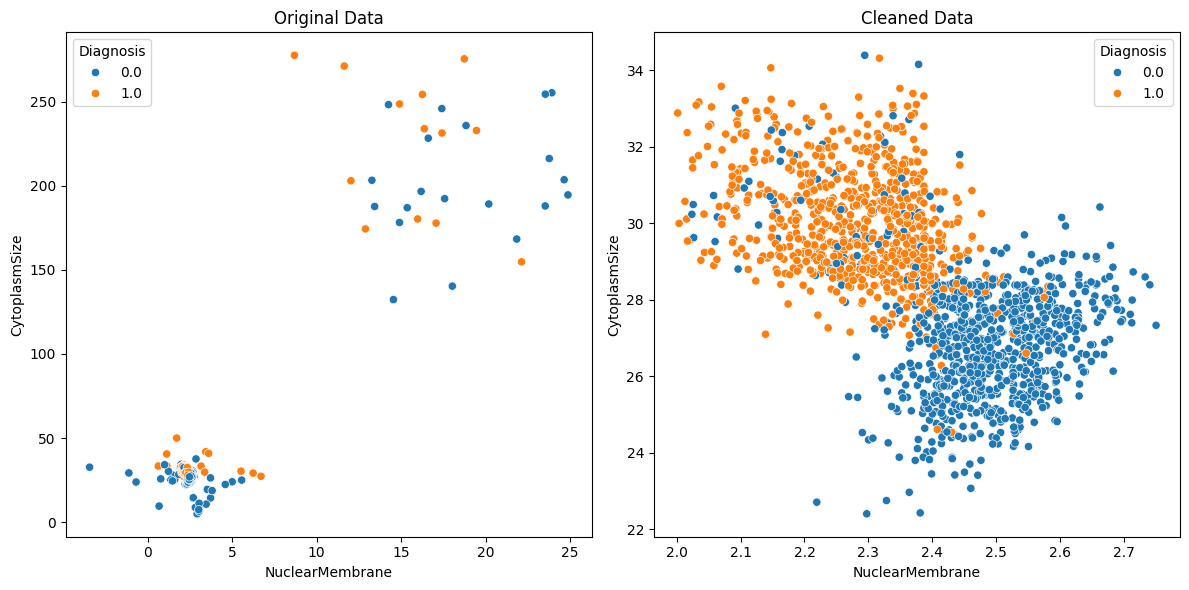
\includegraphics[width=0.8\textwidth]{figures/cleaned_data.png}
    \caption{Distribución y completitud del dataset luego del tratamiento de outliers y valores faltantes.}
    \label{fig:cleaned_data}
\end{figure}

\subsubsection*{Entrenamiento y selección del hiperparámetro $\lambda$}

Una vez completado el preprocesamiento del conjunto de datos, se procedió al entrenamiento del modelo de regresión logística con regularización L2. El objetivo era encontrar el valor óptimo del hiperparámetro $\lambda$ que regula la penalización aplicada a los coeficientes del modelo y permite controlar el sobreajuste.

Para ello, se exploraron dos enfoques complementarios:

\begin{itemize}
    \item \textbf{Barrido de valores}: se entrenó el modelo para un rango logarítmico de valores de $\lambda$, utilizando una partición fija (80\% entrenamiento, 20\% validación). Se midió el F1-score en el conjunto de validación para cada valor de $\lambda$.
    \item \textbf{Validación cruzada ($k=10$ folds)}: se aplicó validación cruzada estratificada repitiendo el entrenamiento y evaluación en diferentes particiones, concatenando las predicciones para obtener una única estimación global del F1-score por cada valor de $\lambda$ (ver sección Métodos).
\end{itemize}

Ambos métodos coincidieron en una región cercana del espacio de búsqueda. Sin embargo, el valor óptimo determinado por el barrido simple arrojó una leve mejora en el rendimiento final del modelo en el conjunto de test. Por esta razón, se optó por continuar utilizando ese valor de $\lambda$ en los experimentos posteriores.

La Figura~\ref{fig:lambda_search} muestra el comportamiento del F1-score a medida que varía el valor de $\lambda$.

\begin{figure}[H]
    \centering
    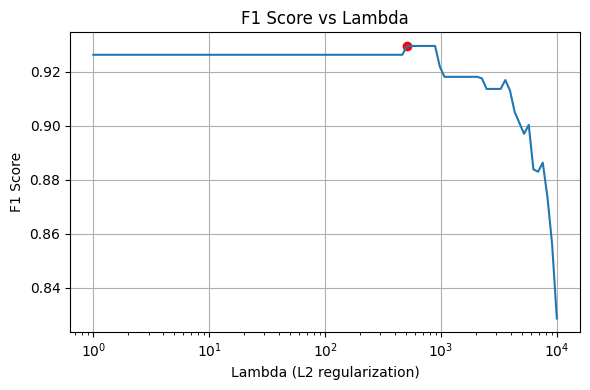
\includegraphics[width=0.75\textwidth]{figures/lambda_search.png}
    \caption{F1-score sobre el conjunto de validación para distintos valores de $\lambda$ explorados mediante barrido logarítmico.}
    \label{fig:lambda_search}
\end{figure}

\subsubsection*{Evaluación sobre el conjunto de test}

Una vez identificado el valor óptimo del hiperparámetro $\lambda$ a través del procedimiento de barrido y validación cruzada, se procedió a entrenar el modelo definitivo sobre el \textbf{conjunto completo de desarrollo balanceado}. A continuación, se evaluó su desempeño sobre el \textbf{conjunto de test balanceado}, que permaneció completamente independiente durante el proceso de ajuste.

Las métricas obtenidas se muestran en la Tabla~\ref{tab:test_metrics}. El modelo logró un rendimiento satisfactorio, manteniendo la coherencia respecto a lo observado en validación. Las curvas ROC y PR correspondientes se presentan en la Figura~\ref{fig:test_curves}.

\begin{table}[H]
    \centering
    \begin{tabular}{lcccccc}
        \toprule
        \textbf{Accuracy} & \textbf{Precision} & \textbf{Recall} & \textbf{F1-Score} \\
        \midrule
        \multicolumn{1}{c}{0.9622} & \multicolumn{1}{c}{0.9419} & \multicolumn{1}{c}{0.9759} & \multicolumn{1}{c}{0.9586} \\
        \bottomrule
    \end{tabular}
    \caption{Desempeño del modelo de regresión logística sobre el conjunto de test balanceado.}
    \label{tab:test_metrics}
\end{table}

\begin{figure}[H]
    \centering
    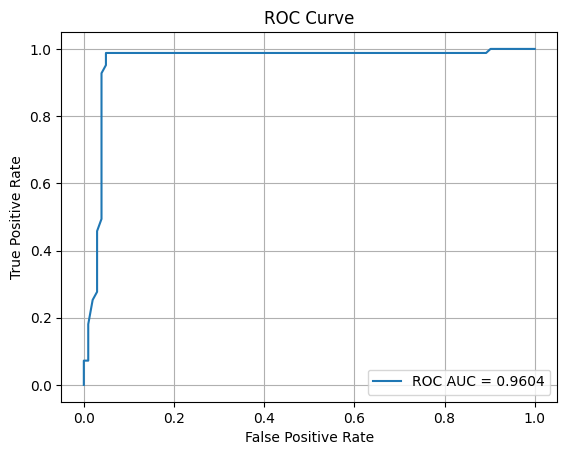
\includegraphics[width=0.32\textwidth]{figures/test_roc.png}
    \hfill
    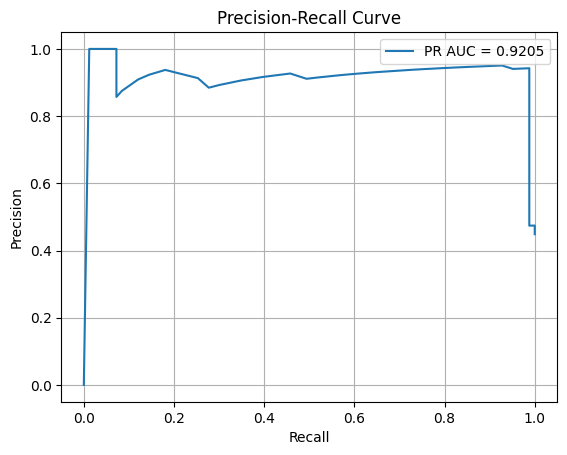
\includegraphics[width=0.32\textwidth]{figures/test_pr.png}
    \hfill
    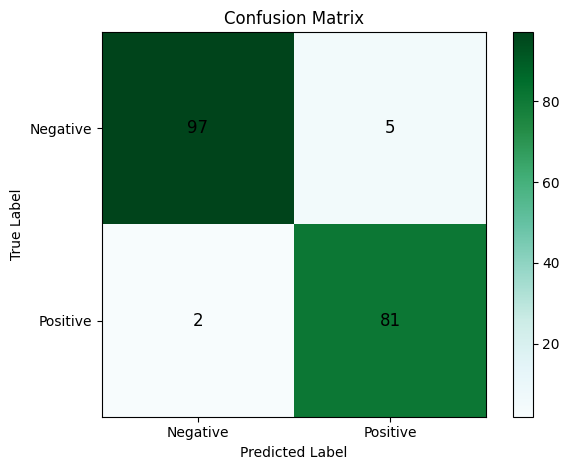
\includegraphics[width=0.32\textwidth]{figures/test_confusion_matrix.png}
    \caption{Curvas ROC (izquierda), Precision-Recall (centro) y Matriz de Confusión (derecha) del modelo evaluado sobre el conjunto de test.}
    \label{fig:test_curves}
\end{figure}

\subsubsection*{Rebalanceo de datos en conjunto desbalanceado}

Para evaluar la robustez del modelo frente al desbalance de clases, se repitió el entrenamiento utilizando el conjunto de desarrollo \textbf{desbalanceado}. En este caso, la proporción entre clases estaba significativamente sesgada, lo que perjudica la capacidad del modelo de detectar correctamente la clase minoritaria.

Se probaron cinco estrategias distintas de rebalanceo, aplicadas antes o durante el entrenamiento:

\begin{itemize}
    \item \textbf{Sin rebalanceo}: el modelo fue entrenado directamente sobre los datos desbalanceados, sirviendo como línea base.
    \item \textbf{Undersampling}: se eliminaron aleatoriamente muestras de la clase mayoritaria hasta igualar la cantidad de muestras de la clase minoritaria.
    \item \textbf{Oversampling (duplicación)}: se replicaron muestras de la clase minoritaria de forma aleatoria hasta alcanzar la misma cantidad que la clase mayoritaria.
    \item \textbf{SMOTE}: se generaron muestras sintéticas de la clase minoritaria mediante interpolación entre instancias cercanas.
    \item \textbf{Cost Re-weighting}: se ajustó la función de pérdida para penalizar más los errores sobre la clase minoritaria, utilizando un peso proporcional a la relación $\frac{\pi_2}{\pi_1}$ entre las probabilidades a priori de ambas clases.
\end{itemize}

Para cada estrategia, se realizó una búsqueda del mejor valor de $\lambda$ utilizando F1-score sobre el conjunto de validación.

\subsubsection*{Evaluación final sobre el conjunto de test}

Luego de seleccionar los hiperparámetros óptimos para cada estrategia de rebalanceo mediante validación cruzada y barrido de $\lambda$, se entrenaron modelos finales utilizando los conjuntos de entrenamiento correspondientes. Estos modelos fueron evaluados sobre el conjunto de test, que se mantuvo completamente separado durante el proceso de ajuste.

La Tabla~\ref{tab:rebalanceo_test_metrics} presenta los valores obtenidos de las métricas principales. Se observa que todos los métodos alcanzan un \textbf{accuracy} idéntico de 0.956, aunque difieren levemente en términos de \textbf{precision}, \textbf{AUC-PR} y \textbf{AUC-ROC}. En particular, la estrategia de \textit{undersampling} logró el mayor F1-score y AUC-PR, mostrando un buen compromiso entre sensibilidad y precisión.

\begin{table}[H]
    \centering
    \resizebox{\textwidth}{!}{%
    \begin{tabular}{lcccccc}
        \toprule
        \textbf{Modelo} & \textbf{Accuracy} & \textbf{Precision} & \textbf{Recall} & \textbf{F1-Score} & \textbf{AUC-ROC} & \textbf{AUC-PR} \\
        \midrule
        Sin rebalanceo         & 0.956 & 0.868 & 0.971 & 0.917 & 0.971 & 0.819 \\
        Undersampling          & 0.956 & 0.850 & 1.000 & 0.919 & 0.970 & 0.825 \\
        Oversampling duplicado & 0.956 & 0.850 & 1.000 & 0.919 & 0.968 & 0.797 \\
        Oversampling SMOTE     & 0.956 & 0.850 & 1.000 & 0.919 & 0.970 & 0.820 \\
        Cost re-weighting      & 0.956 & 0.850 & 1.000 & 0.919 & 0.969 & 0.815 \\
        \bottomrule
    \end{tabular}%
    }
    \caption{Métricas de desempeño final sobre el conjunto de test para distintos métodos de rebalanceo, utilizando los hiperparámetros previamente seleccionados.}
    \label{tab:rebalanceo_test_metrics}
\end{table}

\begin{figure}[H]
    \centering
    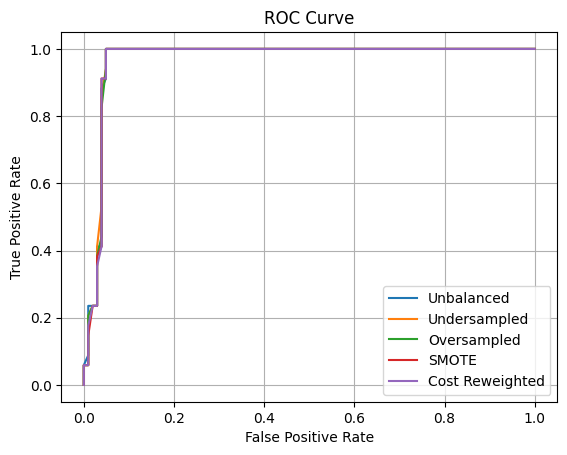
\includegraphics[width=0.32\textwidth]{figures/rebalanceo_roc.png}
    \hfill
    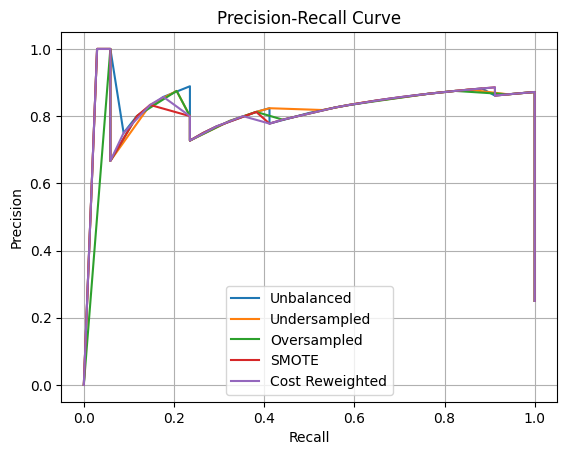
\includegraphics[width=0.32\textwidth]{figures/rebalanceo_pr.png}
    \hfill
    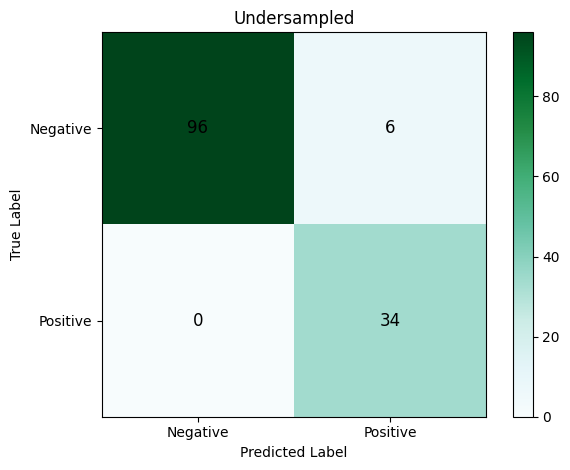
\includegraphics[width=0.32\textwidth]{figures/rebalanceo_conf_matrix.png}
    \caption{Comparación de métricas visuales para las estrategias de rebalanceo evaluadas sobre el conjunto de validación desbalanceado: curva ROC (izquierda), curva Precision-Recall (centro) y matriz de confusión del mejor modelo (derecha).}
    \label{fig:rebalanceo_curves}
\end{figure}

Un aspecto llamativo es que el modelo entrenado \textbf{sin rebalanceo} obtuvo resultados muy similares, e incluso superiores en precisión, respecto a las técnicas específicamente diseñadas para combatir el desbalance. Esta observación se explica por la alta separabilidad inherente de las clases en el espacio de atributos.

Algunas variables presentan una distribución claramente bimodal entre clases, lo que facilita que el clasificador pueda discriminar correctamente incluso en presencia de un fuerte desbalance. Esta estructura puede observarse en la Figura~\ref{fig:scatter_appendix}, incluida en el Apéndice, donde se visualiza la distribución de dos variables numéricas coloreadas por clase.





% EJERCICIO 2
\section{Predicción de Rendimiento de Jugadores de Basketball}
\begin{abstract}
En esta segunda parte del trabajo se abordó un problema de clasificación multiclase, cuyo objetivo fue predecir la categoría de rendimiento (\textit{WAR class}) de un jugador de basketball a partir de sus estadísticas individuales. Se trabajó con un conjunto de datos reales compuesto por múltiples features numéricas y categóricas. Se implementaron y evaluaron distintos clasificadores, incluyendo regresión logística multiclase, LDA y Random Forest.

El conjunto de datos fue preprocesado mediante imputación por KNN y normalización gaussiana. Se utilizaron técnicas de validación cruzada y búsqueda de hiperparámetros para optimizar el rendimiento. Finalmente, se compararon los modelos utilizando métricas multiclase como macro-F1, precisión y recall. El modelo de Random Forest obtuvo el mejor desempeño global, superando a los clasificadores lineales tanto en precisión como en robustez.
\end{abstract}


% INTRODUCCION
\subsection{Introducción}

El objetivo de esta parte del trabajo fue desarrollar un modelo de clasificación multiclase para predecir el rendimiento de jugadores de basketball, a partir de un conjunto reducido pero representativo de estadísticas avanzadas. La variable objetivo es \texttt{WAR class} (Wins Above Replacement class), que segmenta a los jugadores en tres categorías según su impacto en el equipo: rendimiento negativo, nulo o positivo.

Cada instancia del dataset representa el desempeño de un jugador durante una temporada específica, y está caracterizada por las siguientes variables:

\begin{itemize}
    \item \texttt{poss}: número de posesiones en la temporada.
    \item \texttt{mp}: minutos jugados.
    \item \texttt{off\_def}: impacto ofensivo/defensivo global.
    \item \texttt{pace\_impact}: influencia del jugador en el ritmo de juego.
\end{itemize}

Estas métricas combinan aspectos individuales y contextuales del juego, proporcionando una visión condensada del valor del jugador. Dado que la variable objetivo es discreta y toma tres posibles valores, el problema se abordó como una tarea de clasificación supervisada multiclase.

La presencia de desbalance entre clases y la baja dimensionalidad del dataset plantean desafíos tanto para el modelado como para la evaluación. Por ello, se consideraron múltiples arquitecturas, desde modelos lineales hasta métodos basados en árboles, y se utilizaron métricas específicas para clasificación multiclase como el F1-score macro, precisión y recall por clase.



% METODOS
\subsection{Métodos}

Además del modelo de regresión logística multiclase previamente extendido, se incorporaron dos nuevas arquitecturas para abordar el problema de clasificación multiclase:

\paragraph{Análisis Discriminante Lineal (LDA).}
Este método asume que las clases siguen distribuciones normales con una matriz de covarianza común, y busca encontrar combinaciones lineales de las variables que maximicen la separabilidad entre clases. Para una observación $\mathbf{x}$, el clasificador LDA calcula una función discriminante por clase:

\[
\delta_k(\mathbf{x}) = \mathbf{x}^\top \Sigma^{-1} \mu_k - \frac{1}{2} \mu_k^\top \Sigma^{-1} \mu_k + \log \pi_k
\]

donde $\mu_k$ es la media de la clase $k$, $\Sigma$ es la matriz de covarianza común estimada (pooled), y $\pi_k$ es la proporción de muestras de la clase $k$. La predicción se asigna a la clase con mayor $\delta_k(\mathbf{x})$.

\paragraph{Random Forest.}
Se implementó un ensemble de árboles de decisión entrenados sobre distintos subconjuntos bootstrap del conjunto de entrenamiento. Cada árbol fue construido utilizando la entropía como criterio de división, y se combinaron las predicciones por votación mayoritaria.

El clasificador final está compuesto por $T$ árboles $\{h_t\}_{t=1}^T$, y la predicción se obtiene como:

\[
\hat{y} = \text{mode} \left( h_1(\mathbf{x}), h_2(\mathbf{x}), \ldots, h_T(\mathbf{x}) \right)
\]

Este enfoque introduce aleatoriedad tanto en la selección de datos como en la selección de umbrales de división, lo que reduce el sobreajuste y mejora la generalización.

---

Ambos modelos fueron evaluados sobre los mismos datos preprocesados que los modelos lineales. En todos los casos, las predicciones probabilísticas fueron utilizadas para computar métricas como ROC y PR por clase, bajo el esquema \textit{one-vs-rest}.


% RESULTADOS
\subsection{Resultados}

Previo al entrenamiento de los modelos, se realizó un análisis exploratorio del conjunto de datos utilizando nuevamente la extensión \textit{Data Wrangler} \cite{datawrangler2023}. A partir de esta herramienta, se verificó que no existían datos faltantes ni filas duplicadas, lo cual simplificó la etapa inicial de limpieza.

Sin embargo, sí se identificaron valores fuera de los rangos coherentes en varias de las variables numéricas, en particular en \texttt{poss} y \texttt{mp}, las cuales tenian valores negativos (imposibles en este contexto). Estos valores atípicos no eran frecuentes, pero podían comprometer el desempeño de modelos lineales sensibles a escalas y dispersión.

Al igual que en la primera parte del trabajo, se definieron rangos válidos para cada variable basados en la visualización y comprensión de la distribución. Los valores fuera de esos límites fueron marcados como faltantes. Luego, se imputaron utilizando una estrategia por K-vecinos más cercanos ($k=5$), considerando únicamente las instancias válidas como referencia. Esto permitió preservar la estructura del conjunto de datos sin eliminar observaciones ni introducir sesgos arbitrarios.







\bibliographystyle{plain}
\bibliography{referencias}

\appendix
\section{Apéndice}
\subsection{Distribución de variables por clase para datos desbalanceados}

\begin{figure}[H]
    \centering
    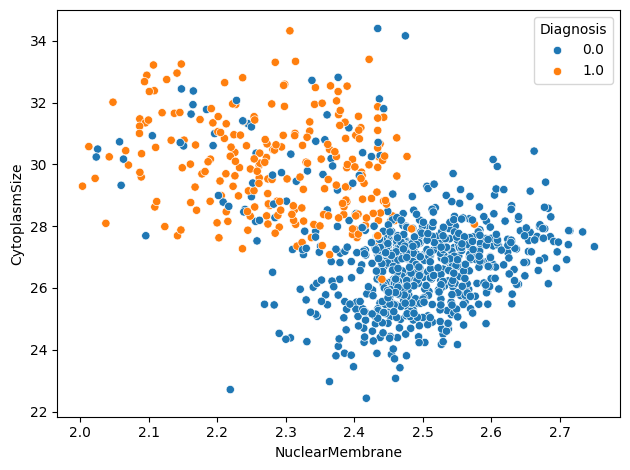
\includegraphics[width=0.6\textwidth]{figures/separability_scatter.png}
    \caption{Visualización de la separación de clases en dos dimensiones. Las clases presentan fronteras bien definidas, lo que explica el alto rendimiento del modelo incluso sin rebalanceo.}
    \label{fig:scatter_appendix}
\end{figure}



\end{document}




